
\chapter{Interpolazione - Infiniti nodi interpolanti}

Il teorema di Faber afferma che non tutti i nodi dell'intervallo converrgono uniformemente
alla funzione che si cerca di approssiamare con infiniti nodi.

\section{Nodi \textit{quasi} Chebichev}
\begin{equation}
x_k^n = \cos \Bigg(\displaystyle\frac{(2k + 1) \pi}{2(n + 1)}\Bigg) \quad k = 0, \dots, n
\end{equation}



\subsubsection{Esempio 5 nodi}
\begin{figure}[h!]
  \begin{center}
    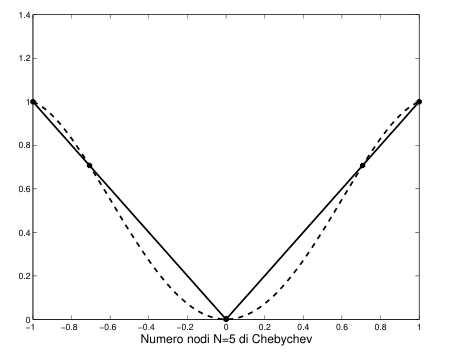
\includegraphics[width=0.3\textwidth]{./images/5_nodi_chebichev.png}
  \end{center}
  \caption{Chebichev con 5 nodi}
  \label{fig:chebichev_5_nodi}
\end{figure}

\subsubsection{Esempio 9 nodi}
\begin{figure}[h!]
  \begin{center}
    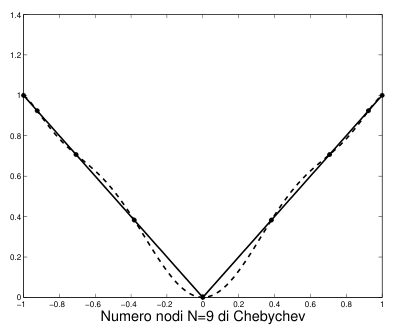
\includegraphics[width=0.3\textwidth]{./images/9_nodi_chebichev.png}
  \end{center}
  \caption{Chebichev con 9 nodi}
  \label{fig:chebichev_9_nodi}
\end{figure}

\subsubsection{Esempio 17 nodi}
\begin{figure}[h!]
  \begin{center}
    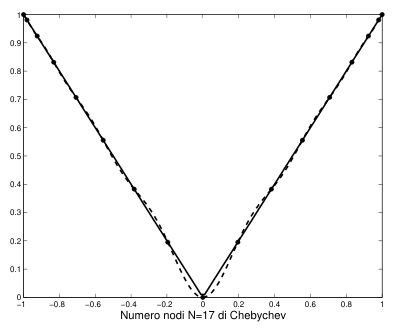
\includegraphics[width=0.3\textwidth]{./images/17_nodi_chebichev.png}
  \end{center}
  \caption{Chebichev con 17 nodi}
  \label{fig:chebichev_17_nodi}
\end{figure}

\section{Convergenza del polinomio di interpolazione}

Il teorema di Bernstein dice che:
\begin{quote}
Se $f(x) \in C^1([a, b])$, il polinomio $p_n(x)$ di interpolazione della funzione f relativo
agli zeri del polinomio di Chebichev di grado $n + 1$ converge uniformemente a $f(x)$ su
$[a, b]$ per $n \rightarrow +\infty$.
\end{quote}



Se la funzione $f \in c^2([a, b])$ si ha che la stima dell'errore è:
\begin{equation}
  || f(x) - p_n(x) ||_{\infty} = O(\displaystyle\frac{1}{\sqrt{n}})
\end{equation}


Se l'intervallo usato per il polinomio interpoaltore è $[0, 1]$ e i nodi sono $n$:

\begin{equation}
  B_{n,k}(x) = \binom{n}{k} x^k (1 - x)^{n - k} \quad k = 0, \dots, n
\end{equation}

Dove:
\begin{equation}
  \binom{n}{k} = \displaystyle\frac{n!}{k! (n - k)!}
\end{equation}


Il teorema di Hermite-Fejer dice che:
\begin{quote}
  Sia $f(x) \in C^0([a, b])$, con $[a, b]$ limitato e chiuso e sia $p_{2n+1}(x)$ 
  il polinomio di grado $2n + 1$ tale che:
\end{quote}
\begin{itemize}
  \item $p_{2n+1}(x_i) = f(x_i)$
  \item $p'_{2n+1}(x_i) = 0$
\end{itemize}


\begin{quote}
  Si ha che gli zeri del polinomio di Chebichev sull'intervallo tendono a zero per infiniti nodi.
\end{quote}
